\RequirePackage{docswitch}
% \flag is set by the user, through the makefile:
%    make note
%    make apj
% etc.
\setjournal{\flag}

\documentclass[twocolumn]{\docclass}

%%%% Scott's macros
\newcommand{\sfig}[2]{
	\includegraphics[width=#2]{#1}
}
\newcommand{\Sfig}[2]{
	\begin{figure}[thbp]
		\sfig{../figures/#1.pdf}{\columnwidth}
		\caption{{\small #2}}
		\label{fig:#1}
	\end{figure}
}
\newcommand{\Swide}[2]{
	\begin{figure*}[thbp]
		\sfig{../figures/#1.pdf}{.8\textwidth}
		\caption{{\small #2}}
		\label{fig:#1}
	\end{figure*}
}
\newcommand{\Sswide}[2]{
	\begin{figure*}[thbp]
		\sfig{../figures/#1.pdf}{.7\textwidth}
		\caption{{\small #2}}
		\label{fig:#1}
	\end{figure*}
}
\newcommand{\Svwide}[2]{
	\begin{figure*}[thbp]
		\sfig{../figures/#1.pdf}{\textwidth}
		\caption{{\small #2}}
		\label{fig:#1}
	\end{figure*}
}

\newcommand{\Spng}[2]{
	\begin{figure}[thbp]
		\sfig{../figures/#1.png}{0.95\columnwidth}
		\caption{{\small #2}}
		\label{fig:#1}
	\end{figure}
}
\newcommand{\Rf}[1]{Figure \ref{fig:#1}}
\newcommand{\rf}[1]{Figure \ref{fig:#1}}
\newcommand{\rsec}[1]{\S\ref{sec:#1}}
\newcommand{\rssec}[1]{\S\ref{subsec:#1}}
\newcommand{\ec}[1]{Eq.~(\ref{eq:#1})}
\newcommand{\ecalt}[1]{Eq.~\ref{eq:#1}}
\newcommand{\Ec}[1]{(\ref{eq:#1})}
\newcommand{\eeec}[3]{Eqs.~(\ref{eq:#1}, \ref{eq:#2}, \ref{eq:#3})}
\newcommand{\eql}[1]{\label{eq:#1}}
\newcommand\be{\begin{equation}}
\newcommand\ee{\end{equation}}
\def\bea{\begin{eqnarray}}
\def\eea{\end{eqnarray}}
\def\svs{\nonumber\\}
\newcommand\full{FCM}
\newcommand\gaussian{GCM}
\newcommand\ctot{\mathcal{C}}

% You could also define the document class directly
%\documentclass[]{emulateapj}

% Custom commands from LSST DESC, see texmf/styles/lsstdesc_macros.sty
\usepackage{lsstdesc_macros}
\newcommand\scott[1]{{\bf [Scott: #1]}}
\newcommand\tassia[1]{{\bf [Tassia: #1]}}
\newcommand\tq[1]{{\bf [Tq: #1]}}
\usepackage{graphicx}
\graphicspath{{./}{./figures/}}
\bibliographystyle{apj}

\usepackage{lineno}
\linenumbers

% Add your own macros here:

% ======================================================================

\begin{document}
	
	\title{Data Compression and Covariance Matrix Inspection: Cosmic Shear}
	\maketitlepre
	
	\begin{abstract}
		Covariance matrices are among the most difficult pieces of end-to-end cosmological analyses. In principle, for two-point functions, each element involves a four-point function, and there are often hundreds of thousands of elements. How best to check these crucial ingredients? Here, we investigate various compression mechanisms, which vastly reduce the size of the covariance matrices in the context of cosmic shear statistics. 
		This helps identify the parts of the covariance matrix that are most significant to parameter estimation. We start with simple compression methods, by isolating and ``removing" 200 modes associated with the highest eigenvalues, then those with the lowest signal-to-noise ratio, before moving on to compression at the tomographic level and, finally, with the Massively Optimized Parameter Estimation and Data (MOPED) algorithm. We find that, while most of these methods proved useful for a few parameters of interest, like $\Omega_m$, the simplest lose constraining power on the intrinsic alignment (IA) parameters as well as $S_8$. %The former was accomplished using a method based on the Karhunen-Lo\'eve (KL) decomposition to obtain the modes with highest SNR, and we show that, in order to reproduce compatible results, we need at least two KL-modes. 
		For the case considered --- cosmic shear from the first year of data from the Dark Energy Survey --- only MOPED was able to reproduce the original constraints in the 16-parameter space. Finally, we apply a tolerance test to the elements of the compressed covariance matrix obtained with MOPED and confirm that the intrinsic alignment parameter $A_{\mathrm{IA}}$ is the most sensitive to inaccuracies in the covariance matrix.
		
		%In this paper, we start along the path of comparing covariance matrices for cosmic shear statistics generated by two different codes. The main goal is to identify the parts of the covariance matrix that are most significant to parameter estimation, and therefore which ones should be calculated more accurately. We engage different ways of doing this, starting with a simple one-to-one comparison of the elements, then moving on to eigenvalues and finally to the signal-to-noise ratio (SNR). In the spirit of reducing the number of relevant elements, we “remove” 200 modes associated with the highest eigenvalues, then those with the lowest SNR. We find that it is not possible to locate the most important elements using the first method but, while the analysis with the SNR proved resourceful for a few parameters of interest, like $\Omega_m$, we lost constraining power on the intrinsic alignment (IA) parameters as well as $S_8$. We also tested ways to shrink the covariance matrix, both at the tomographic level, and for the two-point functions. The former was accomplished using a method based on the Karhunen-Lo\'eve (KL) decomposition to obtain the modes with highest SNR, and we show that, in order to reproduce compatible results, we need at least two KL-modes, but just like in the SNR case, this is not the case for all parameters. Finally, we apply a lossless compression scheme to the covariance matrix, capable of reducing the dimension to the number of free parameters. We were successful in reproducing the constraints obtained previously and show that the elements of the new matrix have an error tolerance of up to $25\%$.
	\end{abstract}
	
	% Keywords are ignored in the LSST DESC Note style:
	\dockeys{}
	
	\maketitlepost
	
	% ----------------------------------------------------------------------
	% 
	
	\section{Introduction}
	\label{sec:introduction}
	
	Cosmic shear is a weak lensing effect caused by the large-scale structure of the universe and is an important tool for constraining cosmology. The most common way of extracting information about cosmology from cosmic shear is to use two-point functions; as is often the case, such analysis uses a covariance matrix. For a two-point data vector of length $N$, the covariance matrix is a symmetric $N\times N$ matrix with $N\times (N+1)/2$ individual elements that capture the auto and cross-correlation of the data vector. As the data vector increases, the number of elements in the covariance matrix grows quadratically and becomes harder to analyse. One could potentially speed up computations and provide a simpler method of analysing the covariance matrix by using compression schemes capable of significantly reducing the size of the matrix while still retaining relevant information about the parameters of interest. One way of obtaining this is to use the Massively Optimized Parameter Estimation and Data (MOPED) algorithm, in which, if the noise in the data does not depend on the model parameters, the compression is lossless in the sense that the Fisher matrix is the same for both the full and the compressed covariance matrices \cite{Heavens:2000hjl, Tegmark:1997maa}. MOPED has been widely used in literature for a variety of topics, like, for example, analysing CMB data \cite{Zablocki:2015zcm}, for redshift space galaxy power spectrum and bispectrum \cite{Gualdi:2018mjl}, for parameter-dependent covariance matrices \cite{Heavens:2017smv}, for compressing the Planck 2015 temperature likelihood \cite{Heather:2019d} and, more recently, it has been paired with a Gaussian Process emulator to analyse Weak Lensing data \cite{Mootoovaloo:2020}.
	
	We will focus on cosmic shear measurements from the Dark Energy Survey (DES)~\cite{Troxel:2017xyo} Year 1 release; the data vector has 227 elements, varying with angular separation, and different pairs of tomographic redshift bins. Since our parameter space consists of 16 free parameters, we can use MOPED to reduce the $25,878$ independent elements of the covariance matrix, to only $136$.
	
	Apart from MOPED, we will also be analysing the covariance matrix with three other compression methods: the first involves discarding the modes associated with the highest eigenvalues; the second method removes those with the lowest signal-to-noise ratio. In an effort to shrink the covariance matrix to about $10\%$ of its original size, we remove, in both cases, 200 such modes.
	
	Finally, the third method consists of a map-level compression \citep{Alonso:2017hhj}, where linear combinations of the tomographic maps are used to retain as much information as possible. Compression of the tomographic bin pairs then considerably reduces the size of the data vector of the two-point functions. For example, we will see that most of the information in the four tomographic bins used by DESY1 can be compressed into a single linear combination of those bins. Therefore, instead of $(4\times5)/2$ two-point functions for each angular bin, we need include only one.
	For this purpose, the tomographic bins will have the same length, and so the angular cuts to the dataset and covariance matrix will be different from the ones used in the aforementioned DESY1 paper. The chosen covariance matrix has a dimension of $190 \times 190$, and so, for one eigenmode, we can compress it to $10\%$ of its original size, yielding 190 independent elements.
	
	In \rsec{methods}, we start by describing the dataset and the covariance matrices used. We then proceed to review each compression scheme and apply them to DESY1 cosmic shear.  The ultimate test is how well they reproduce the constraints obtained with the full covariance matrix.
	We follow up by showing that compression can be a useful tool to compare two different covariance matrices, in \rsec{comparison_matrices}.
	Our tolerance test is described in \rsec{tolerance}, where we test what happens to the parameter constraints when we introduce noise to elements and eigenvalues separately. Finally, our conclusions are summarised in \rsec{conclusion}.
	
	%The next three sections walk through increasingly complex ways of determining the most important parts of these matrices: we start with an element by element comparison of  the two covariance matrices in \rssec{comparison_one-one}, then move on to look at the eigenvalues in \rsec{eigenvalues}, and, finally we use the signal-to-noise ratio in \rsec{snr}. We validate our findings by comparing them with the constraints obtained with the unmodified covariance matrix. %In \rssec{comparison_one-one}, we compare element by element of the two covariance matrices . In \rsec{eigenvalues},  we use eigenvalue as a way to compare the covariance matrices. In \rsec{snr}, we calculate the signal-to-noise ratio and use it to compare the covariance matrices. %We will use this metric a bit throughout but want to state here that our goals is to simply finding out that two covariance matrices give different results is a black-box approach. One cannot identify the source of the disagreement. The methods described here aim to be a bit deeper to try to understand where the key differences arise and which differences are most important. (this is ambiguous)
	
	%A simple compression method is applied in both \rsec{eigenvalues} and \rsec{sec:snr}, where we discard 200 modes of the covariance matrix associated with the highest eigenvalues, then those with lowest signal-to-noise ratio, respectively. We apply more complicated compression schemes in  \rsec{sec:shrinkage}, using techniques developed by Alonso \citep{Alonso:2017hhj} and by Tegmark and Heavens \citep{Tegmark:1997maa}, capable of reducing the dimension to the number of free parameters, thus obtaining  a compression ratio of 1\%. Our tolerance test is described in \rsec{tolerance}, where we compare what happens to the parameter constraints when we introduce noise to elements and eigenvalues separately. Finally, our conclusions are summarised in \rsec{conclusion}.
	
	%Another goal of this work is to explore the shrinkage of the covariance matrices. In \rsec{eigenvalues} and \rsec{snr}, we discard 200 modes of the covariance matrix associated with the highest eigenvalues, then those with lowest signal-to-noise ratio. In \rsec{eigenvalues}, we tested two novel compression scheme and manage to apply a lossless compression scheme capable of reducing the dimension to the number of free parameters, achieving a compression ratio of 1\% for the covariance matrices.
	
	% ----------------------------------------------------------------------
	\section{Methods}
	\label{sec:methods}
	
	\subsection{DES Cosmic Shear: Data and Analysis}
	\label{subsec:data_and_analysis}
	
	In this section, we introduce the data and covariance matrices that are used in this work. Our tests are carried out using cosmic shear statistics $\xi_\pm(\theta)$, focusing on the Year 1 results of the Dark Energy Survey \citep{Troxel:2017xyo,Abbott:2018cms} (DESY1). The data is divided into four tomographic redshift bins spanning the interval $0.20 < z < 1.30$, which yields 10 bin-pair combinations, each one containing 20 angular bins between 2.5 and 250 arcmin. We thus begin with 200 data points for each $\xi_+(\theta)$ and $\xi_-(\theta)$, giving 400 in total. We then apply the angular cuts described in \citep{Abbott:2018cms}, which removes the scales most sensitive to baryonic effects; this leaves 167 points for $\xi_+(\theta)$ and 60 for $\xi_-(\theta)$, resulting in 227 data points corresponding to the aforementioned $227 \times 227$ covariance matrix. 
	
	Table~\ref{tab:priors} shows the 16-parameters varied and the priors placed on them. To perform cosmological parameter inference we use the {\tt CosmoSIS} \citep{Zuntz:2015med, Lewis:2000taj, Kirk:2012mnras, Kilbinger:2009aa, Howlett:2012jcap, Bridle:2007njp, Takahashi:2012taj, Smith:2003mnras} pipeline, while employing the {\tt MultiNest} \citep{Feroz:2009fhb} sampler to explore the parameter space, with 1000 {\tt livepoints}, {\tt efficiency} set to 0.05, {\tt tolerance} to 0.1 and {\tt constant efficiency} set to True.
	
	\begin{table}
	\centering
	\begin{tabular} { l c} 
		\hline
		\hline
		Parameter		& Prior	\\ \hline
		Cosmological    & \\ [1ex]
		$\Omega_m$      & $\mathcal{U}(0.1, 0.9)$ \\
		$\log A_s$      & $\mathcal{U}(3.0, 3.1)$ \\
		$H_0 \mathrm{(km s^{-1} Mpc^{-1})}$	& $\mathcal{U}(55, 91)$\\
		$\Omega_b$      & $\mathcal{U}(0.03, 0.07)$ \\
		$\Omega_\nu h^2$& $\mathcal{U}(0.0005, 0.01)$ \\
		$n_s$           & $\mathcal{U}(0.87, 1.07)$ \\ [1ex]
		\hline
		Astrophysical       & \\ [1ex]
		$A_{\mathrm{IA}}$	& $\mathcal{U}(-5, 5)$ \\
		$\eta_{\mathrm{IA}}$& $\mathcal{U}(-5, 5)$ \\ [1ex]
		\hline
		Systematic      & \\ [1ex]
		$m^i$			& $\mathcal{G}(0.012, 0.023)$ \\
		$\Delta z^1$	& $\mathcal{G}(-0.001, 0.016)$ \\
		$\Delta z^2$	& $\mathcal{G}(-0.019, 0.013)$ \\
		$\Delta z^3$	& $\mathcal{G}(0.009, 0.011)$ \\
		$\Delta z^4$	& $\mathcal{G}(-0.018, 0.022)$ \\ [1ex]
		\hline
		\hline
	\end{tabular}
	\caption{List of the priors used in the analysis for parameter constraints ($\mathcal{U}$ denotes flat in the given range and $\mathcal{G}$ is gaussian with mean equal to its first argument and dispersion equal to its second). For the cosmological parameters, we fix $w = -1.0$, $\Omega_k =  0.0$ and $\tau =  0.08$. The astrophysical parameters are associated with the intrinsic alignment, they follow the relation $A_{\mathrm{IA}}(z) = A_{\mathrm{IA}}[(1+z)/1.62]^{\eta}$. Lastly, for systematics we have $m^i$ corresponding to the shear calibration and  $\Delta z^i$ for the source photo-$z$ shift, with $i = 1, 4$ in both cases.}
	\label{tab:priors}
	\end{table}
	
	
	The covariance matrices used are the following:
	\begin{itemize}
		\item the Full Covariance Matrix (\full) used in the DESY1 analysis, which includes non-gaussian effects and super-sample variance; it was generated by {\tt Cosmolike} \citep{Krause:2016jvl};
		\item one containing only the gaussian part, which we will refer to as the Gaussian Covariance Matrix (\gaussian).
	\end{itemize}
	Thus, throughout, the covariance labels \full\ and \gaussian\ differ for several reasons: first, they are two independent codes (\gaussian\ is generated by the same code used to analyse the KiDS-450 survey \citep{Kohlinger:2017sxk})
	and, second, although the code for the KiDS-450 survey does contain all the functionality in {\tt Cosmolike}, we ran with the simplest settings in order to accentuate the differences. The ensuing larger differences will help us assess various validation techniques. Where not otherwise stated, the analysis and constraints will be performed on \full.
	
	\rf{Y1-constraints_wmS8A} shows the results for the projected cosmological constraints for \full\ and \gaussian, using the same data vector and cuts. The $2\sigma$ constraints are as follows: for \full: $\Omega_m= 0.306^{+ 0.073}_{- 0.060}$, $A_{\mathrm{IA}} = 0.852^{+ 1.005}_{- 1.086}$ and $S_8 = 0.784^{+ 0.200}_{- 0.171}$; and for \gaussian: $\Omega_m = 0.309^{+ 0.073}_{- 0.058}$, 	$A_{\mathrm{IA}} = 0.948^{+ 0.916}_{- 0.985}$ and $S_8 = 0.787^{+ 0.196}_{- 0.166}$. This shows that the differences we have introduced to the calculation of the two matrices are measurable in the parameter constraints.
	
	\Sfig{Y1-constraints_wmS8A}{Constraints on cosmological parameters $\Omega_m$ and $S_8$ and intrinsic alignment parameter $A_{\mathrm{IA}}$ for two covariance matrices produced for cosmic shear. The purple curve is for \full\ while the blue is for \gaussian. In the 16--dimensional parameter space, the volume of the posterior is about $22\%$ larger for the former.}
	
	% -------------------
	\subsection{Eigenvalues}
	\label{subsec:eigenvalues}
	
	Let us start with the easy task of analysing the eigenvalues of the covariance matrix. Each eigenvalue is associated with a linear combination of the data vector, or a \emph{mode}.
	
	The lowest eigenvalues correspond to modes with the smallest variance but since they are not normalised, it is unclear how this variance compares to the signal in the mode. Let us nonetheless explore the possibility that the modes with the lowest variance provide the most information and therefore dropping the ones with the largest eigenvalues would not affect the final result.
	
	Our procedure consists of first diagonalising the covariance matrix in order to calculate its eigenvalues and then replacing the large eigenvalues with a larger number (nine orders of magnitude higher), thus removing their effective contribution; we then transform back to the original basis and perform a cosmological analysis with the new covariance matrix, to constrain the parameters of our model. 
	
	In order to reduce the covariance matrix to about 10\% its original size, we follow the procedure above to discard the 200 eigenmodes with the largest eigenvalues, \rf{EigSNR-constraints_wmS8A} shows the results obtained.  The constraints are significantly broader for the three parameters shown. This is consistent with the fact that we are reducing about 90\% of the information contained in the covariance matrices. However, it is inconsistent with the notion that they are irrelevant, in fact, constraints on $S_8\equiv \sigma_8 (\Omega_m/0.3)^{0.5}$ for the original covariance matrix are $0.784^{+ 0.200}_{- 0.171}$, whereas, for this procedure, we obtain $0.679^{+ 0.533}_{- 0.505}$, showing an increase in the errors of almost 200\%. It is then clear that a different way of ordering the modes, other than simply looking at the eigenvalues, is called for.	
	
	\Sfig{EigSNR-constraints_wmS8A}{Constraints on cosmological parameters $\Omega_m$, $S_8$ and the intrinsic alignment parameter $A_{\mathrm{IA}}$ for the original covariance matrix (in purple) and for the two new covariance matrices obtained in \rssec{eigenvalues} (in blue) and \rssec{snr} (in magenta).}
	
	\Svwide{SNR_cuts200}{Scatter plot for the relation between the signal to noise (SNR)  for each parameter (y-axis) against that for the full set of parameters (x-axis). The derivatives are shown with respect to $\Omega_m$ (blue circle), for $S_8$ (orange \textbf{x}) and for the intrinsic alignment parameter $A_{\mathrm{IA}}$ (green triangle). The purple rectangle spreads until the two hundred lowest values of SNR, which corresponds to the values that are modified for parameter constraints.}
	
	% -------------------
	\subsection{Signal-to-noise ratio}
	\label{subsec:snr}
	
	Instead of looking only at the ``noise'' -- or the eigenvalues of the covariance matrix -- a better way to assess the importance of modes is to consider the signal as well. We can define the expected signal-to-noise ratio (SNR) as
	\be
	\left(\frac{S}{N}\right)^2 = \sum_{ij} T_i C^{-1}_{ij} T_j\
	,\ee
	where $T_i$ is the predicted theoretical signal for the $i^{th}$ data point, given a fiducial cosmology, and $C$ is the covariance matrix. If $C$ were diagonal, then the eigenvectors would simply be the $T_i$s themselves, as opposed to a linear combination of them, and we could estimate the SNR squared expected in each mode by just computing $T_i^2/C_{ii}$. Then we could throw out the modes with the lowest SNR. Since $C$ is not diagonal, we have to first diagonalise it and then order the values. So, we write the expected SNR squared as
	\bea
	\left(\frac{S}{N}\right)^2
	&=& \sum_{i} \frac{v_i^2}{\lambda_i}\
	,\eea
	where $\lambda_i$ are the eigenvalues of the covariance matrix, which is diagonalised with the unitary matrix $U$, and the eigenvectors are 
	\be
	v_i\equiv U_{ij}^T T_j\
	.\ee
	From a naive point of view, this makes it clear which modes should be kept and which should be dropped; modes $v_i$ for which $v_i^2/\lambda_i$ is small can be discarded. As we will later see, however, it is not as simple as that.
	
	After obtaining the SNR for the covariance matrix, we proceed to set the 200 lowest values to seven orders of magnitude lower, which is equivalent to increasing the noise (or decreasing the signal) of these modes. We then obtain a new covariance matrix with the corresponding modified SNR values. 
	The parameter constraints for this method are shown in \rf{EigSNR-constraints_wmS8A}, where we note that only $\Omega_m$ is well constrained (in agreement with those obtained with the original covariance matrix to within a $2\sigma$ interval). The constraining power on $A_{\mathrm{IA}}$ and $S_8$, on the other hand, is very much lost, which suggests that the modes removed do indeed carry relevant information for these parameters.
	
	We can investigate this loss by tweaking our understanding of which modes carry information. The ``signal'' that these modes are ordered by is the amplitude of the data points.  The parameters , however, are sensitive to the shape as well as the amplitude.
	To address this, we can identify the SNR for each parameter individually by taking
	\bea
	\left(\frac{\partial S/\partial p_\alpha}{N}\right)^2 = \sum_{i} \frac{(\partial v_i / \partial p_\alpha)^2}{\lambda_i}\
	,\eea
	where $\partial /\partial p_\alpha$ is the derivative with respect to each parameter. This produces the SNR for each parameter of interest. The importance of this procedure is illustrated in \rf{SNR_cuts200}, which shows the normalised SNR for a given mode on the $x$-axis and the SNR for each parameter for the same mode for $\Omega_m$, $S_8$ and $A_{\mathrm{IA}}$. The shaded region shows the 200 modes excluded in the previous analysis, so we clearly see that there are some low SNR modes there that contain information about the parameters. This is particularly true for the intrinsic alignment parameter $A_{\mathrm{IA}}$, which seems to explain the poor constraints shown in \rf{EigSNR-constraints_wmS8A}. As a result, simply cutting on raw SNR loses constraining power.
	
	This analysis was also applied to the 200 modes with the highest SNR, and found similar results. While \citeauthor{Louca:2020} (2020) argues that this would be recommended in order to obtain a bias-free inference (another way would be to use a non-Gaussian likelihood), we believe that our results diverge only due to the large quantity of modes that were removed for our purposes.
	
	% -------------------
	\subsection{Tomographic Compression}
	\label{subsec:tomographic_compression}
	
	This compression method is based on a Karhunen-Lo\'eve (KL) decomposition for the shear power spectrum suggested by \citep{Alonso:2017hhj} and later applied to real space two-point function in \citep{Bellini:2019ssw} for CFHTLens survey. This method finds the eigenmode --- in this case, a linear combination of the convergence in different tomographic bins --- with most of the signal-to-noise ratio contribution to the power spectrum, and then transforms the two-point function of this eigenmode into real space. This method is not the most general compression method for the two-point function in real space, since the weight is $\ell-$dependent. However, as found in \citep{Bellini:2019ssw}, it is effective on the real space data nonetheless. 
	
	Before delving into the derivation, it is worth summarizing the results. With {\tt CosmoSIS}, we calculate the shear power spectrum $C_{\ell}$ of the convergence $\kappa^i$ in the 4 tomographic bins probed by DES Year 1 with a fiducial cosmology at the best-fit parameters. With 4 bins, there are $4\times 5/2=10$ pairs of bins for which we can compute spectra. The left plot in \rf{ClDl} shows the diagonal elements of the signal part and the noise part of the spectrum. The right-hand panel shows the spectrum of the modes with the largest signal to noise, ranging from $\ell = 10$ to $\ell = 2500$. That is, we identify a mode as $b_{\ell m} = \sum_i w_i \kappa_{\ell m}^i$, where the sum is over the 4 bins with a weighting factor that we will discuss below. For each $\ell$, the right panel shows the top KL-transformed eigenmodes, which we will call $D_{\ell}$. We can see that the first KL mode contains most of the SNR contribution to the power spectrum. However, if we want to recover more information, we also should include the second and the cross mode between the first and second KL-mode.
	
	\begin{figure*}[thbp]
	    \sfig{figures/Cl_newrange.png}{0.8\columnwidth}
		\qquad \qquad \qquad
	    \sfig{figures/Dl_newrange.png}{0.8\columnwidth}
		\caption{\textbf{Left:} Shear power spectrum of \full. Solid lines are diagonal elements of the signal matrix $S_{\ell}$, and dashed lines are the diagonal elements of noise matrix $N_{\ell}$.
		\textbf{Right:} Signal-to-noise ratio matrix $D_\ell$ of KL-modes of the power spectrum on the left.  \label{fig:ClDl}}
	\end{figure*}
	
	With  {\tt CosmoSIS}, we generate the shear power spectrum $C^{ij}$ of the convergence $\kappa^i$ for the fiducial cosmology, which is the best-fit value of the DES Year 1 results for cosmic shear only. With the total power spectrum $\ctot=C+N$, the sum of the signal and shape noise $N$, we can calculate the Karhunen-Lo\'eve (KL) modes for each $\ell$ (so we drop the $\ell$ subscript) via a general eigenvalue problem 
	\be
	\ctot^{ij} e^j_p = \Lambda_p N^{ij} e^j_p
	.\ee
	The index $p$ in $e_p^i$ corresponds to the $p^{th}$ KL-mode of $\ctot$. Using Cholesky decomposition, $N = L L^{\dagger}$, the new observable can be expressed as $b_p = e_p^i  L^{-1}_{ij} \kappa_{j}$. We should note that $C_{\ell}$ is the angular power spectrum of the weak lensing shear, and $E_{\ell}$ is similar to a transformation of basis so that the shear signal is orthogonalized. Afterwards, we can now calculate the power spectrum $D_{\ell}$ for the new observable $b_{\ell m}$ for each $\ell$
	\be
	D_{\ell} =\ \langle b_{\ell m} b_{\ell m}^T \rangle \ = E_{\ell} L^{-1} \ctot_{\ell} L^{-1} E^{T}_{\ell}\
	,\ee
	or, if we denote $E_{\ell} N^{-1}$ as $R_{\ell}$ and further denote $U_{\ell}^{ij}=R^i_{\ell} R^j_{\ell}$, we can write the compression in one simple linear combination of the $C_{\ell}$,
	\be
	D_{\ell} = R_{\ell}^i C_{\ell}^{ij} R_{\ell}^j = U_{\ell}^{ij} \ctot_{\ell}^{ij}\
	.\ee
	$U_{\ell}^{ij}$ is the weight on the tomographic bin-pair, which we can later use to compress the two-point functions. We should point out that these KL-modes are uncorrelated, so the power spectrum of the new observable $D_{\ell}$ is a diagonal matrix, with 1+SNR of the corresponding eigenmodes on the diagonal elements. Since the KL-decomposed modes of shear power spectrum are uncorrelated, we can make a compression here by taking only the first one or two modes with the highest SNR. By doing so, we compress ten tomographic bin-pairs to one or two.
	
	We want, however, to eventually compress the two-point function data vector of DESY1, which is measured is real space and related to the angular power spectrum $C_{\ell}$ via
	\begin{equation*}
	\xi_{\pm}^{ij}(\theta) = \int \frac{\ell d \ell }{2\pi}J_{0/4}(\ell \theta) C^{ij}(\ell)\ 
	.\end{equation*}
	In order to use only a linear combination of all the tomographic bins, we need to make sure that the combination is $\ell$-independent, that is to say, the two-point correlation function corresponding to $D_{\ell}$, $\Tilde{\xi}_{\pm}(\theta)$, can be directly calculated from other two-point functions. In \rf{kl-mode}, we show that compression matrices $U^{ij}(\ell)$ are generally $\ell$-independent, except for low $\ell$s, because of the existence of cosmic variance. Therefore, we have, 
	\bea
	\nonumber\Tilde{\xi}_{\pm}(\theta) &=& \int \frac{\ell d \ell }{2\pi}J_{0/4}(\ell \theta) D(\ell)\\\nonumber
	&=&\int \frac{\ell d \ell }{2\pi}J_{0/4}(\ell \theta) U^{ij})\ell C^{ij}(\ell)\\
	&=&U^{ij}\xi_{\pm}^{ij}(\theta)\
	,\eea
	where $U^{ij}$ is the average $U^{ij}_{\ell}$ weighted by the number of multipoles for each $\ell$ that is $2\ell+1$
	\be
	U^{ij} = \frac{\int_{\ell _{\mathrm{min}}}^{\ell _{\mathrm{max}}} d\ell\, (2 \ell +1) U^{ij}_{\ell}}{\int_{\ell _{\mathrm{min}}}^{\ell _{\mathrm{max}}} d\ell\, (2 \ell +1)}\
	.\ee
	We make a more conservative angular cut than the one discussed in \cite{Troxel:2017xyo}, making sure that both $\xi_{\pm}$ are uniform in regard to tomographic combinations. We consider an angular scale for  $\xi_+$ from $7.195'$ to $250.0'$, and for $\xi_-$ from $90.579'$ to $250.0'$. Therefore, for the purpose of exploring the KL-transform, the raw data vector has a length of 190. By shrinking 10 tomographic combinations for each angle into 1 KL-mode, the data vector is shrunk to length 19, and so the number of elements in the covariance matrices are reduced by 99\%.
	
	\begin{figure*}[thbp]
	    \sfig{figures/epi.png}{0.8\columnwidth}
	    \sfig{figures/Wij.png}{1.02\columnwidth}
		\caption{\textbf{Left:} Normalised KL-eigenmodes $E_\ell^p$ of the shear power spectrum $C_{\ell}$, the changes in shades represent different $\ell$. \textbf{Right:} Transformation on tomographic bin combination $U_{ij}$ constructed by the KL-eigenmodes. Black lines are the weighted average of each mode. The lightest color for each mode represent $\ell = 10$ and increase by $\Delta \ell = 10$ for each step toward darker color. \label{fig:kl-mode}}
	\end{figure*}
	
	In \rf{kl-mode}, we plot the normalised KL-eigenmode $E_\ell^i$ of $C_{\ell}$ and its corresponding $U^{ij}_\ell=R_\ell^i R_\ell^j$. Modes with increasing $\ell$ are plotted in increasing darkness of the colour. We can see that the KL-modes do not depend significantly on the scale factor $\ell$, so we also take the weighted average of the eigenmodes $E_\ell^p$ and its quadratic form $U_\ell$ over $\ell$'s and plot them with black lines. 	We see that for different $\ell$, the KL-modes do vary by a slight amount. For the first KL-mode, the tomographic bins with higher redshift are weighted more than those with low redshift. This is also shown in the right panel by the weight on tomographic combination that the combination of bin 3 and bin 4 carries most of the weight in the signal-to-noise ratio. This agrees with the fact that low-redshift galaxies are less affected by lensing than high-redshift galaxies, as indicated in the left panel of \rf{ClDl}.
	
	\begin{figure}[b]
		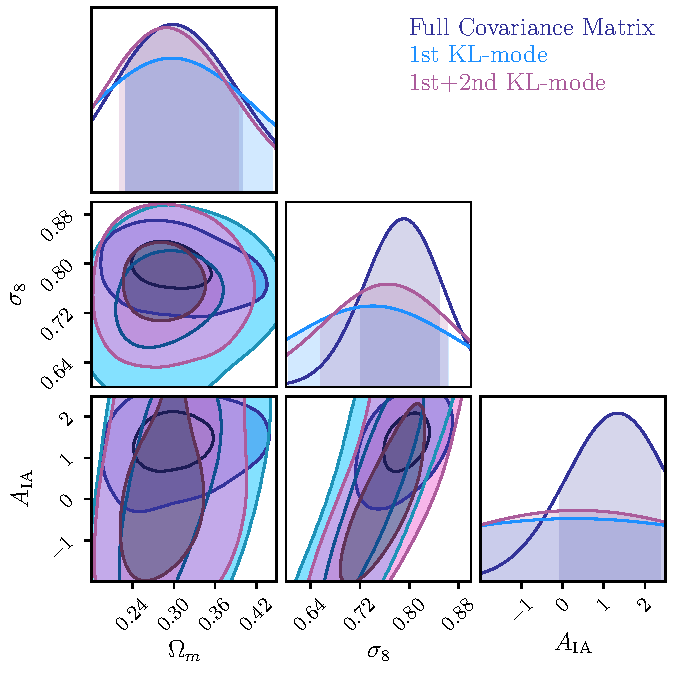
\includegraphics[width=\columnwidth]{CompKL-constraints_wmS8A.pdf}
		\caption{Cosmological constraints marginalised over all 16 parameters for the  $190 \times 190$ \full\ and that compressed by the first KL-mode and the first two KL-modes.\label{fig:CompKL-constraints_wmS8A}}
	\end{figure}
	
	We ran the likelihood analysis with the first KL-mode and the first two KL-modes with their cross correlation mode, which correspond to a 10-to-1 and 10-to-3 compression, respectively, and show the parameter constraints on the $\Omega_m - S_8 - A_{\mathrm{IA}}$ plane in \rf{CompKL-constraints_wmS8A}. We can see that the first KL-mode is generally not sufficient to recover the information in the data vector. Since the first two modes contain most of the SNR contribution at a map level, we were able to recover the $\Omega_m$ constraints. However, information about the $S_8-A_{\mathrm{IA}}$ combination is clearly lost. This could be due to the fact that the SNR-prioritised modes are not the sensitive direction for these parameters, as was also the case in \rf{SNR_cuts200}. Indeed, the $S_8 - A_{\mathrm{IA}}$ plane shows a strong correlation between these two parameters. This likely explains why the $S_8$ constraints got wider: the KL-modes fail to break the degeneracy on $A_{\mathrm{IA}}$, which is mostly contained in the modes that are insensitive to cosmic shear, and are discarded in the compression process.
	
	% -------------------
	\subsection{Applying MOPED}
	\label{subsec:2pt_compression}
	
	\Svwide{Weights_2pt}{An illustration of the 227 values of the weights corresponding to $\Omega_m$, $S_8$ and $A_{\mathrm{IA}}$ used for compressing the covariance matrices. Note how similar the weighing vectors for $S_8$ and $A_{\mathrm{IA}}$, and that the largest values for correspond to the last 60 elements, i.e. these will be used to compress the part of the covariance matrix that holds information for $\xi_-$.}
	
	The compression here takes place at the two-point level, with the compressed data vector containing linear combinations of the many two-point functions. In principle, this requires only $N_p$ linear combinations of the two-point functions where $N_p$ is the number of free parameters, and each mode, or linear combination, contains all the information necessary about the parameter of interest. 
	
	For each parameter $p_\alpha$ that is varied, one captures a single linear mode
	\be
	y_\alpha = U_{\alpha i} D_i\
	,\ee
	where $D_i$ are the data points and the coefficients are defined as
	\be \label{eq:compression_scheme}
	U_{\alpha i} \equiv \frac{\partial T_j}{\partial p_\alpha} \, C^{-1}{}_{ji}\
	,\ee
	with $T_j$ being the theoretical prediction for the data point $D_j$ for a fiducial cosmology. An illustration of the matrix $U_{\alpha i}$ is shown in \rf{Weights_2pt}, showing the weighting vector for parameters $\Omega_m$, $S_8$ and $A_{\mathrm{IA}}$.
	
	The now much smaller data set $\{y_\alpha\}$, which contains $N_p$ data points, carries its own covariance matrix, with which $\chi^2$ can be computed for each point in parameter space. Propagating through shows that this covariance matrix is related to the original $C_{ij}$ via
	\be
	C_{\alpha\beta} = U_{\alpha i} C_{ij} U^T_{j\beta}\ 
	,\ee
	which also happens to be identical to the Fisher matrix of our likelihood. This compression was first suggested by \citeauthor{Tegmark:1997maa} (1997) for a single parameter only.  The non-trivial extension to multiple parameters, where the full Fisher matrix is reproduced with the compressed data, is the MOPED algorithm \citep{Heavens:2000hjl}. One difference here is that our weighing vector given by \ec{compression_scheme} does not carry the normalising factor of Eq. (11) in \citep{Heavens:2000hjl}.
	It is worth noting that compression does not automatically speed up the computation for parameter inference, since it has to be redone for every point in the parameter space. Recent work has been done by \cite{Mootoovaloo:2020} to address this problem by using Gaussian Processes to generate the compressed theory.
	
	The covariance matrix used here is  $227 \times 227$, while the number of parameters needed to specify the model is only 16, so $C_{\alpha\beta}$ is a $16\times 16$ matrix. We have apparently captured from the initial set of $(227 \times 228)/2 = 25,878$ independent elements of the covariance matrix a small subset (only 136) of linear combinations of these 26k elements that really matter. If two covariance matrices give the same set of $C_{\alpha\beta}$, it should not matter whether any of the other thousands of elements differ from one another.
	
	Ultimately, what matters is how well the likelihood does at extracting parameter constraints. Since most analyses assume a Gaussian likelihood, this boils down to how well the contours in parameter space agree when computing $\chi^2$ using two different covariance matrices.	
	
	\rf{Comp2pt-constraints_wmS8A} compares the constraints obtained for the compressed covariance matrix and data set with results from the full one. The two curves agree extremely well for the parameters shown: $\Omega_m$, $S_8$ and $A_{\mathrm{IA}}$. This is also true for all the other cosmological and intrinsic alignment parameters, where their mean values agree at the $2 \sigma$ confidence level. While the volume of the whole constrained parameter space does increase by about 13\%, the constraints for most parameters are less than 4\% broader, which shows that the information loss is negligible. 
	
	\Sfig{Comp2pt-constraints_wmS8A}{Constraints on cosmological parameters $\Omega_m$ and $S_8$ and for the intrinsic alignment parameter $A_{\mathrm{IA}}$ for the original covariance matrix, \full, (in purple) and for the compressed one (in blue).}
	
	% ----------------------------------------------------------------------
	\section{Comparison of Covariance Matrices}
	\label{sec:comparison_matrices}
	
	Armed with this information about compression, we now set out to compare the two covariance matrices, \gaussian\ and \full, described in \rssec{data_and_analysis}. 
	
	\subsection{Element-by-element comparison}
	\label{subsec:compare_one-one}
	
	We begin by performing an element-by-element comparison between the two covariance matrices. If there were only a single data point, then the covariance matrix would be one number and comparing two covariance matrices to try to understand why they give different constraints would be as simple as comparing these two numbers.  The simplest generalisation is then to do an element-by-element comparison. We make a scatter plot of the elements of the two matrices in the bottom panel of \rf{Y1-scatter}, where we can see that the elements of \full\ are, in general, larger than \gaussian's, with many of the off-diagonal elements differing by 2 orders of magnitude or more.
	In some ways, this is useful and reassuring, as it aligns with what we see in the parameter constraints, in \rf{Y1-constraints_wmS8A}: larger elements in the covariance matrix translates to less constraining power. 
	
	The limitation of this method is that it remains unclear which of the differences are driving the final discrepancies in parameter constraints. This difficulty is an outgrowth of the increasing size of the data sets and hence the growing number of elements of the covariance matrix that any two codes are likely to disagree on. This element-by-element comparison, however, would prove much more useful if we fewer elements to compare. Towards that end, we turn to compressed covariance matrices.
	
	\Sfig{Y1-scatter}{In both plots, the red points refer to the diagonal elements, and the colour bar varies according to the number of elements in one hexagonal bin, where the darkest blue colour corresponds to only one element, and the brightest yellow shade to 2000. \textbf{Top:} Scatter plot of the ratio of the elements of \gaussian\ and \full\ vs the \full\ value. For illustrative purposes, we draw a black, horizontal line at \gaussian/\full = 1. \textbf{Bottom:} Density of the scatter plot of the positive elements of the \gaussian\ and \full, with the black line showing \full\ = \gaussian.}
	
	% -------------------
	\subsection{Compressed Matrices Comparison}
	\label{subsec:compare_compressed}
	
	\begin{figure}[b]
		\sfig{Comp2pt-scatter}{0.85\columnwidth}
		\caption{{\small Results for the covariance matrices compressed following the procedure described in \rssec{2pt_compression}, with the red points corresponding to the diagonal elements.
		\textbf{Top:}  One-to-one scatter of the ratio of the elements of \gaussian\ and \full, over elements of \full. The black horizontal line is drawn at \gaussian/\full\ = 1.
		\textbf{Bottom:}  One-to-one scatter of the elements of the compressed matrices, with the black line describing \full\ = \gaussian.}}
		\label{fig:Comp2pt-scatter}
	\end{figure}
	
	Since we have shown that, among all compression schemes shown here, the only one capable of reproducing the original parameter constraints was MOPED, that is what we will be using in this section.
	
	We compress both covariance matrices using the same $U_{\alpha, i}$ (we also tried using different $U$'s for each and obtained similar results).
	%Here, we take two different approaches: first, we assume that $U_{\alpha, i}$ is the same for both covariance matrices and we calculate it with CL. The second approach is that each compression scheme must use the original covariance matrix that will be compressed, so that $U_{\alpha, i}$ will be different for each covariance matrix. We find that the mean values of the parameter constraints for the two methods both agree to $> 2\sigma$ of the original constraints. It is also crucial that the matrices used for comparison here are those obtained via the same compression scheme, so that we can be sure that their differences are indeed only related to the differences in the original matrices. 
	\rf{Comp2pt-scatter} show a one-to-one scatter plot, which, as expected, exhibits a similar behaviour to that observed in \rf{Y1-scatter}, with the elements of \full\ being larger than those of \gaussian. Here, however, the ratio of the diagonal elements is closer to 1, and the ratio of the diagonal elements goes up to only $\approx 2.3$. Perhaps even more importantly, there are much fewer points on this plot, meaning that MOPED reduces the number of elements that need to be compared. These figures provide a greater insight into the relevant elements for parameter estimation: the dispersion is largely damped, and most of the elements are within $25\%$ of each other, which explains what we see in the parameter constraints. \rf{Comp2pt-correlation} shows the correlation matrix for \gaussian\ and \full, and the difference between the normalized off-diagonal elements. The small differences suggest that the root of the slightly looser constraints obtained with \gaussian\ is the larger diagonal elements of the MOPED-reduced covariance matrix. That is, a problem that initially required inspecting hundreds of thousands of elements is reduced to one involving only 16.
	
	\Sfig{Comp2pt-correlation}{The upper right and lower left plots display the correlation matrix for \gaussian\ and \full\ respectively, and the difference between them, $\Delta r_{ij}$, is shown on the lower right.}
	
	% ----------------------------------------------------------------------
	\section{Tolerance of the Compressed Matrices}
	\label{sec:tolerance}
	
	\Svwide{Tolerance_constraints}{An error plot showing the changes to the constraints for $\Omega_m$, $S_8$ and $A_{\mathrm{IA}}$ for errors added at $5\%, 10\%, 15\%, 25\%, 30\%, 35\%, 40\%$ and $45\%$ of the original elements (in purple) and eigenvalues (in green) of the compressed covariance matrix. The blue rectangle covers the $2 \sigma$ interval obtained for the original \full, and the green line shows the mean value for the respective parameter.}
	
	Now that we have shown that we are indeed able to compress the covariance matrix into a much simpler and considerably smaller one, our next step is to analyse the amount of error the elements can tolerate while reproducing compatible parameter constraints.
	
	In the next two sections we test two different ways of perturbing the covariance matrix: first we consider an error to the elements themselves, then we follow a similar procedure to study the effects of introducing error to the eigenvalues of the compressed covariance matrix. In both cases the perturbation is drawn in the following manner: consider that we want to test the impact of an error $x \%$; this can either be an increase of a decrease in the original element, or eigenvalue, such that what we care about most is not whether the parameter constraints will be larger, but rather how different. For this error to be random, but centred at our desired percentage, we draw $\delta$ from a Gaussian distribution, $\mathcal{G}(0,\frac{x}{100})$ and calculate the new value to be
	\be \label{eq:tolerance}
	C_{\alpha \beta}^{\mathrm{new}} = (1 + \delta)C_{\alpha \beta}^{\mathrm{old}}\ 
	,\ee
	where, for the eigenvalue, we replace $C_{\alpha \beta}$ with $\lambda_i$. This analysis is done only for \full, with errors ranging from $5 - 45 \%$, and for 50 realizations of the perturbed matrices.
	
	One of the concerns that arises when modifying the covariance matrix is that the resulting one has to be positive definite (PD), as such, in each section we also describe the steps taken to ensure this. Another intelligent way of guaranteeing PD would be to perturb the log of the covariance matrix. One of the issues that arises, however, is how to introduce an error to the log matrix that would be similar to what we expect to see in the original covariance matrix -- introducing a $10\%$ error, for example, in such a matrix results in a perturbed covariance matrix with elements several orders of magnitude higher than the original one. A safer procedure would then be to perturb the log of its eigenvalues, but, since we have a section dedicated to perturbations to the eigenvalues themselves, we deemed this would be repetitive.
	
	% -------------------
	\subsection{Modifying the elements}
	
	Once we generate new values for each independent element, following \ec{tolerance}, we check for positive definiteness. Since the resulting matrix is, more often than not, not PD, we correct this by identifying the smallest negative eigenvalue and adding it to the diagonal \cite{Yuan:2008}. We check that, although doing this largely increases the values of the diagonal elements, only less than $40 \%$ have a standard deviation of more than twice the original perturbation. 
	
	The constraints for $\Omega_m$, $S_8$ and $A_{\mathrm{IA}}$ are shown in \rf{Tolerance_constraints}, in purple, where the blue rectangle spans over the constraints for the unchanged compressed covariance matrix. It is interesting to note that, while the relative change in size for the $2\sigma$ interval is $> 8 \%$ for the cosmological parameters, this goes up to $\sim 80 \%$ for the intrinsic alignment parameter $A$.
	
	% -------------------
	\subsection{Modifying the eigenvalues}
	
	Another way of introducing error to the covariance matrix is to perturb its eigenvalues. For a symmetric matrix, we have
	\be
	C_{\alpha \beta} = Q\Lambda Q^{-1}\ 
	,\ee
	where $\Lambda = \lambda I$, with $\lambda$ being the eigenvalues and $I$ the identity matrix; and $Q$ is a square matrix whose columns are composed of the eigenvectors of $C_{\alpha \beta}$. The eigenvalues are then perturbed as described in \ec{tolerance}, and the error, $\delta$ is drawn from $\mathcal{G}(0,\frac{x}{100})$, with the requirement that $|\delta| < 1$. We then have $\lambda^{\mathrm{new}} > 0$, and thus the perturbed covariance matrix associated with these new eigenvalues is PD. 
	
	The results for this method are also plotted in \rf{Tolerance_constraints}, in green. Despite the results following the same tendency as those of the last section, we find that about $80\%$ of the elements of the perturbed covariance matrices are within $10\%$ of their original value. This shows that the intrinsic alignment parameter $A$ is very sensitive to errors in the covariance matrix.
	
	% ----------------------------------------------------------------------
	\section{Conclusion}
	\label{sec:conclusion}
	
	In this work, we set out to explore different ways of compressing, comparing and analysing covariance matrices, giving particular emphasis to MOPED. We started off looking at the parameter constraints of two $227 \times 227$ covariance matrices \full\ and \gaussian, generated for DESY1 cosmic shear measurements, and saw that, although some of their elements differed by several orders of magnitude, they generated similar constraints. It was clear, then, that not all elements contribute equally to the parameter constraints, and we needed to employ increasingly complicated methods to try and locate the most relevant parts of the covariance matrix.
	
	The first step was then to analyse the eigenvalues. We began with the hypothesis that modes associated with the lowest eigenvalues have the lowest variance and therefore carry most information, as such, those with the highest eigenvalues would contribute less to parameter estimation. Using this notion to compress the covariance matrix yielded worse constraints: ``removing" the highest 200 eigenvalues, by setting them to nine orders of magnitude higher resulted in an increase of about 200\% in the size of the $2 \sigma$ constraints. Next, we moved on to the signal-to-noise ratio, and, using a similar procedure adopted for the eigenvalues, we ``removed" the modes with the lowest SNR. The results showed us that these modes did not contribute significantly to constraining some cosmological parameters, like $\Omega_m$, but constraints on the intrinsic alignment parameters, and even $S_8$ were considerably affected. This is consistent with the fact that the IA parameters are more sensitive to low SNR in cosmic shear, and it shows us that we need to look at the SNR per parameter before making any cuts, so that we do not lose important information for the parameters that we want to constrain.
	
	The next step was to shrink the covariance matrix by applying a tomographic compression, where we decompose the shear angular power spectrum into KL modes, then we look for modes with the highest SNR and compress shear data vector by the modes. We thus go from ten tomographic bin combinations to only one or two. The resulting covariance matrix, for one mode, is then reduced from $190 \times 190$ to $19 \times 19$ or $59 \times 59$, showing a reduction of about $99\%$ or $91\%$, respectively. We show, however, that one mode is not sufficient for constraining the parameters of our model, with the results being similar to our previous tests involving SNR: the constraints for $\Omega_m$, for example, are reproduced with the first and second KL-mode, but this is not the case for the IA parameters. Since essential information of IA parameters is contained in low SNR KL-mode, the high KL-modes failed to break the degeneracy of $A_{\mathrm{IA}}-S_8$ correlation, resulting in wider $S_8$ constraints. 
	
	Finally, we applied MOPED, which uses linear combinations of the data vector. By transforming the data vector and covariance matrix with a weighting vector that is parameter dependent, we were able to reduce the $227 \times 227$ matrix to a $16 \times 16$, and since the Fisher matrix is identical for both the original and compressed ones, the compression scheme is lossless. This is also clear in the parameter constraints, where we show that we are able to reproduce the similar constraints for the two matrices, for all parameters. On the other hand, we compared the elements of the compressed covariance matrix for \full\ and \gaussian\ and found that the new elements show reasonable agreement, with their correlation matrices being very similar, and the diagonal elements showing a percentage difference of less than $15\%$.
	
	Given these results, we successfully show that MOPED is the only compression scheme, out of the ones considered in this work, capable of capturing all the relevant information required to reproduce reliable parameter constraints for the 16 parameters of interest.
	
	When looking at \rf{Y1-scatter}, the large variance in the element-by-element comparison suggests that there could be considerable differences in the parameter constraints. We see, however, in \rf{Y1-constraints_wmS8A}, that this is not the case. This becomes clearer when comparing the elements of the compressed covariance matrices, where, while they do follow the same tendency as the full comparison, only a smaller portion of the elements display a greater dispersion.
	
	One last step was taken to analyse the error tolerance of the compressed \full. We adopted two ways of doing this, by introducing error taken from a Gaussian distribution for $5 - 45 \%$ of the original 1) element and, 2) eigenvalue of the compressed covariance matrix. For the latter, we checked that only about $20 \%$ of elements of the resulting, perturbed, covariance matrix showed errors within the expected value, while the vast majority had only about a $10\%$ error. In both cases, however, the results were similar: for the cosmological parameters $\Omega_m$ and $S_8$, the $2\sigma$ constraints changed by less than $8\%$, while the constraining power for intrinsic alignment parameter $A_{\mathrm{IA}}$ was largely lost. This result is repeated throughout this work: we find that most modifications made to the covariance matrix greatly affect $A_{\mathrm{IA}}$, with the exception of MOPED. It is, therefore, advised that extra precaution be taken when performing compression methods, if this parameter is to be considered.

	%\textcolor{red}{Finally, in the sense of applicability, our results are encouraging for methods which seek to speed up calculations for parameter estimation using MOPED, such as by using Gaussian Processes to produce the coefficients $U_\alpha$ from \ec{compression_scheme} \cite{Mootoovaloo:2020}.}
	
	% ----------------------------------------------------------------------
	% ----------------------------------------------------------------------
	\subsection*{Acknowledgments}
	
	The authors wish to thank Sukhdeep Singh and Hung-jin Huang for useful discussions.
	
	%%% Here is where you should add your specific acknowledgments, remembering that some standard thanks will be added via the \code{desc-tex/ack/*.tex} and \code{contributions.tex} files.
	
	%This paper has undergone internal review in the LSST Dark Energy Science Collaboration. % REQUIRED if true
	
	
 
	
	T.F. and T.Z. contributed extensively writing the main paper as well as implementing the covariance comparison and compression. N.C. contributed to the compression code. All authors participated in the discussion and gave valuable suggestions.
	
	% Standard papers only: author contribution statements. For examples, see http://blogs.nature.com/nautilus/2007/11/post_12.html
	
	% This work used TBD kindly provided by Not-A-DESC Member and benefitted from comments by Another Non-DESC person.
	
	% Standard papers only: A.B.C. acknowledges support from grant 1234 from ...
	
	The DESC acknowledges ongoing support from the Institut National de Physique Nucl\'eaire et de Physique des Particules in France; the Science \& Technology Facilities Council in the United Kingdom; and the Department of Energy, the National Science Foundation, and the LSST Corporation in the United States.  DESC uses resources of the IN2P3 Computing Center (CC-IN2P3--Lyon/Villeurbanne - France) funded by the Centre National de la Recherche Scientifique; the National Energy Research Scientific Computing Center, a DOE Office of Science User Facility supported by the Office of Science of the U.S.\ Department of Energy under Contract No.\ DE-AC02-05CH11231; STFC DiRAC HPC Facilities, funded by UK BIS National E-infrastructure capital grants; and the UK particle physics grid, supported by the GridPP Collaboration.  This work was performed in part under DOE Contract DE-AC02-76SF00515.
 % also available: key standard_short
	
	%		\appendix
	\section{Invertible Transformation and Tolerance Testing}
	
	In the last section, we shrink the data vector and covariance matrices and find the most cosmological-informative modes in both. However, in order to make a tolerance testing of each element in the covariance, we not only need the cosmological-informative modes but also the uninformative modes. Suppose we find the informative set of modes for cosmology, the modes that are orthogonal to them, or the complementary set of the informative one, form a set of modes that are cosmological-uninformative. 
	
	To find these modes, we start off with the compression scheme presented in Eq. \ref{eq:compression_scheme}, which will serve as the basis for a rotation matrix $W_\alpha$. We then use the Gram-Schmidt decomposition to create $227 - N_p$ vectors orthonormal to $U_{\alpha}$, thus obtaining a unitary $227 \times 227$ matrix. We then have,
	\be
	C'_{\alpha\beta} = W_{\alpha i} C_{ij} W^T_{j\beta}.
	\ee
	%When this transformation is applied to the original matrix, $C_{ij}$, the first $N_p \times N_p$ elements of the new matrix will be the same as we had in $C_{\alpha\beta}$. Since our transformation spreads out the information contained in the compressed matrix, the relevant values for parameter estimation will be contained in the first $N_p$ rows and columns of the new covariance matrix. This means that we will have $N_p \left( 2 \times 227 - N_p \right)$ important elements, which is about an order of magnitude less than in the case of the full covariance matrix.
	
	\begin{figure}[]
		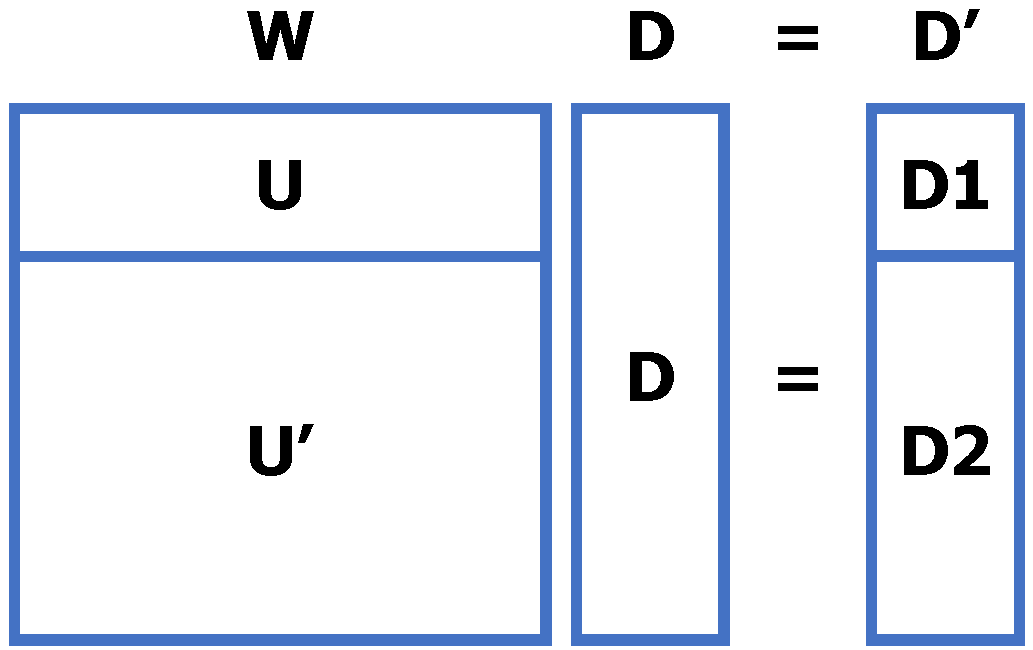
\includegraphics[width=0.45\columnwidth]{Transformation_data.pdf}
		
		\bigskip
		
		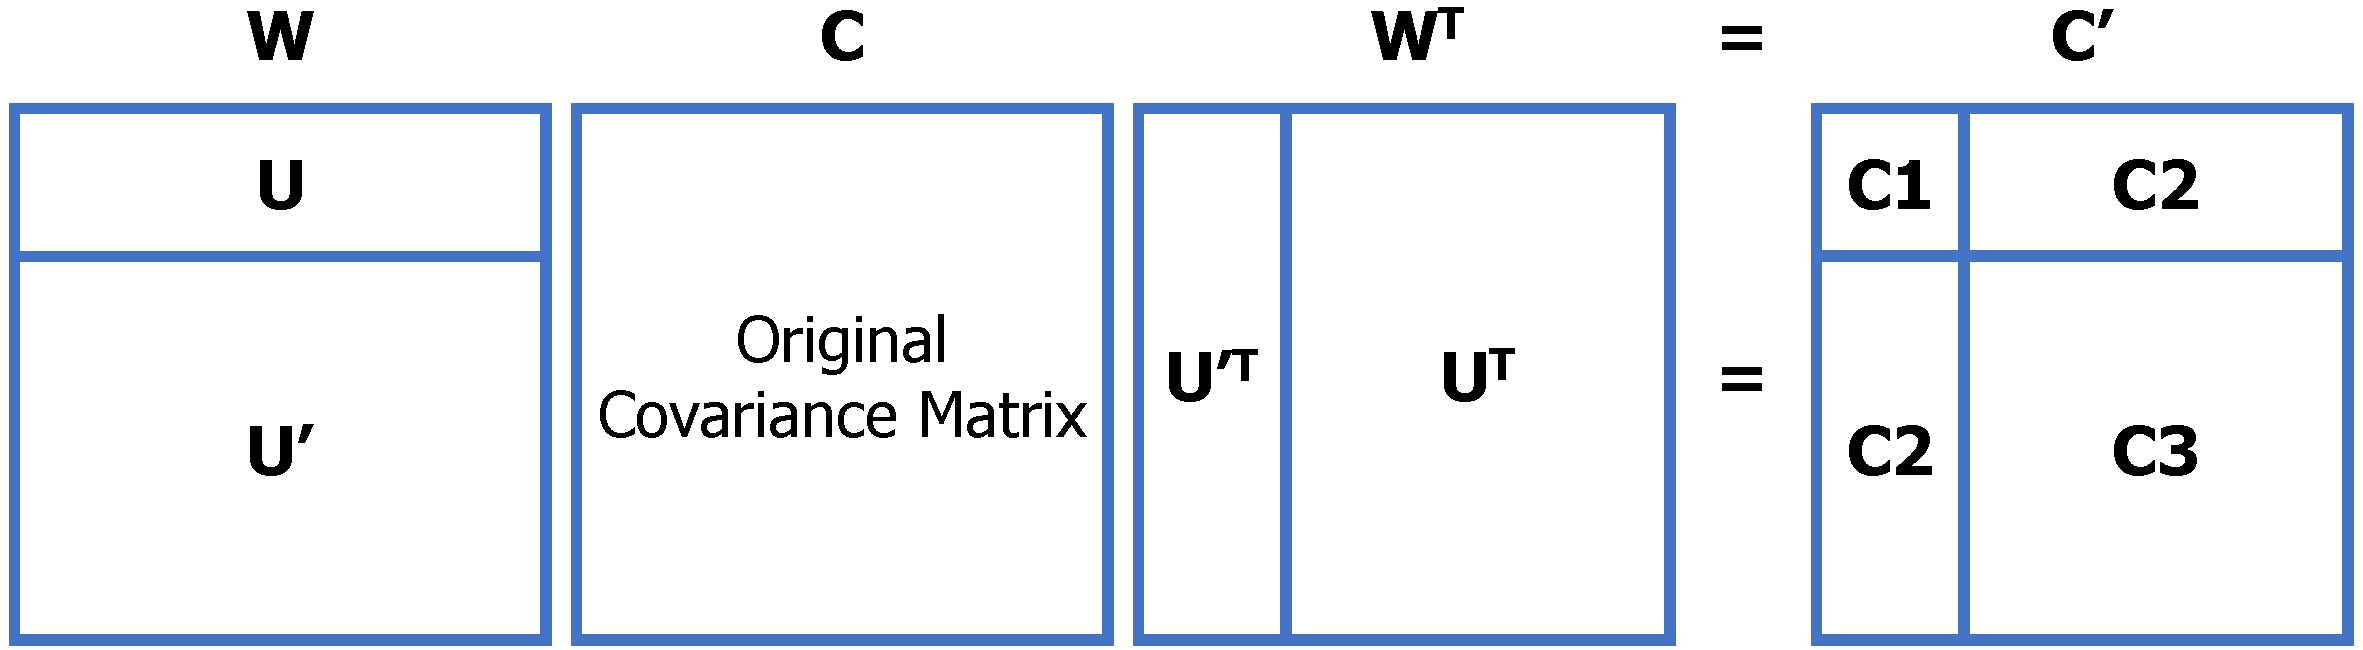
\includegraphics[width=0.99\columnwidth]{Transformation_CM.pdf}
		\caption{Illustration of the invertible transformation, $W$. It's components, $U$ and $U'$ are the compression scheme described in Sections \ref{subsec:shrinkage} and orthogonal components obtained using the Gram-Schmidt decomposition, respectively. \textbf{Top:} Transformation of the data vector, where D1 corresponds to compressed set, and D2 are uninformative for parameter constraints. \textbf{Bottom:} Transformation of the covariance matrix. The last square on the right, $C'$ is divided into four blocks: C1 is the most informative to cosmology, C2 are also relevant to constraints, but on a lower scale, and, finally, C3 is irrelevant to the $\chi^2$ calculation. \label{fig:transformation}}
	\end{figure}
	
	With the invertible transformation $W$, shown in \figref{transformation}, the data vector and covariance matrix are transformed into sectional blocks. We will describe the meaning of each block here. The data vector is split into two blocks: D1 has the transformed data points that are sensitive to changes in the cosmological parameters, that is, the cosmological-sensitive data; D2 is generated by the modes that are orthogonal to D1, they will, in principle, be unaffected by changes to the cosmological parameters, which makes them uninformative for parameter constraints.
	
	The transformed covariance matrix is split into 4 blocks, with the off-diagonal ones being the transpose of each other. Block C1 is the variance and covariance of the cosmological-sensitive data, D1, it describes how well the cosmological-sensitive data is measured, and is, therefore, the one that contributes most to the $\chi^2$ calculation, and, consequently, to parameter constraints. Block C2 is the cross-correlation between D1 and D2, it is important for parameter constraints because it describe how D1 is affected by the uncertainty of D2.  Finally, C3 relates to the uninformative data, D2; it plays a minor role to $\chi^2$, so it affects the parameter constraints least.
	
	%With this invertible transformation W shown in \figref{illu-trans}, the data vector and covariance matrix are transformed into sectional blocks. We will describe the meaning of each blocks here. The data vector is split into two blocks. D1 is the block of transformed data points that are sensitive to the changes in cosmological parameter set, that is, the cosmological-sensitive data. D2 is generated by the modes that are orthogonal to the cosmological sensitive mode, they will in principle stays relatively constant when cosmological parameter changes and are uninformative for parameter constraints.
	
	%The transformed covariance matrix is split into 4 blocks, with the off-diagonal blocks being the transpose of each other, there are 3 different blocks. Block C1 is the variance and covariance of the cosmological informative data, or D1. This block contributes almost everything to the $\chi^2$ calculation. C1 describes how well the cosmological-sensitive data is measured, so the value in this block will affect the parameter constraints. Block C2 is the variance and covariance of the uninformative data, or D2. It plays a minor role in the $\chi^2$, so it will affect the parameter constraints less. C3 is the cross-correlation between D1 and D2, and it will affect the parameter constraints because it describes how D1 is affected by the uncertainty of D2.
	
	The next step is then to test the tolerance of different parts of the transformed covariance matrix. We first compare the results of increasing the error of each block separately by a factor of 100 and compare the results to constraints with the unmodified covariance, then we start by introducing smaller errors to the relevant blocks, C1 and C2 and analyse the corresponding increase in the parameter constraints.
	
	\section{Tolerance Testing}
	
	Given that block C1 contains the same elements as those in the compressed covariance matrix, it is intuitive to think that this is the only block relevant for parameter constraints. It is clear, however, in 	\figref{tolerance1000} that this is not the case. Multiplying the elements of blocks C1 and C3 do not alter the constraints, whereas changes made to blocks C2 and C1+C2 do. To explain this, we need to look at what happens to $\chi^2$ when using the transformed data set and covariance matrix. We have
	\be
	\chi^2 = \mathbf{(D - T)\ C^{-1}\ (D-T)}^t
	, \ee
	where $\mathbf{C}^{-1}$ is the inverse of the covariance matrix, $\mathbf{D}$ is the data set and $\mathbf{T}$ is the theory prediction (in our case, for $\xi_+$ and $\xi_-$). If we take the simple case of a $3 \times 3$ matrix,
	\be
	\mathbf{C} = 
	\left( \begin{matrix}
		\mathrm{C1} & \mathrm{C2} & \mathrm{C2} \\
		\mathrm{C2} & \mathrm{C3_{11}} & \mathrm{C3_{12}} \\
		\mathrm{C2} & \mathrm{C3_{21}} & \mathrm{C3_{22}} \\
	\end{matrix} \right)
	\ee
	and
	\be
	\mathbf{(D - T)} = 
	\left( \begin{matrix}
		p \\
		q \\
		q
	\end{matrix} \right)
	,\ee
	then,
	\be \label{eq:chi2}
	\chi^2 = \frac{p^2 \mathrm{det(C3)} + \left(q^2 \mathrm{C1}\ - 2pq \mathrm{C2}\  \right)(\Delta C3)}{		
		\mathrm{C1\ det(C3) - C2^2\ (\Delta C3)}}
	,\ee
	for
	\be
	\mathrm{det(C3) = C3_{11}\ C3_{22} - C3_{12}\ C3_{21}}
	,\ee
	and
	\be
	\mathrm{\Delta C3 = C3_{11} - C3_{12} - C3_{21} + C3_{22}}
	,\ee
	where $\mathrm{C3}_{12} = \mathrm{C3}_{21}$.

We find that while the form of $\chi^2$ for our $227 \times 227$ covariance matrix is greatly more complicated than Eq. \ref{eq:chi2}, it follows a similar structure: terms from block $\mathrm{C1}$ are multiplied by block $q^2$, block $\mathrm{C2}$ by $pq$, and, finally, $\mathrm{C3}$ multiplies $p^2$ and the other two blocks.

If we recall that blocks $\mathrm{C3}$ and $q$ do not hold any relevant information about the original covariance matrix and data set, then it is clear why changes made to $\mathrm{C3}$ do not affect the parameter constraints. In fact, even if we are to multiply this block by a very large number, $\chi^2$ would be reduced to only $p^2$, and the constraints would not alter.

On the other hand, if we increase the elements of $\mathrm{C1}$, then we would be left with only $q^2$, which has no information about the data, and therefore we would lose constraining power. This is clearly what happens for a small, $3 \times 3$ covariance matrix. Remember, however, that in our real case, $\mathrm{C1}$ has only 136 independent elements, whereas $\mathrm{C2}$ has 25 times as many. Increasing block $\mathrm{C_1}$, then does not necessarily cancel out the terms multiplying $p$ and C2, and since the former carries important information, our constraints do not change. This becomes clearer when we look at the terms that make up the denominator of $\chi^2$: if we take the dimension of the covariance matrix to be $n$, then the fraction of terms multiplied by elements of $\mathrm{C2}$ follows the sequence $\frac{n-1}{n}$, which means that 99.56 $\%$ is composed of terms with $\mathrm{C2}$. Therefore while the block $\mathrm{C1}$ is indeed the most relevant (in the $16 \times 16$ case these are all the elements we need for obtaining compatible constraints as with the full covariance matrix), altering it in the transformed matrix produces no apparent changes to the constraints.
	
	%\be
	%v_i^\alpha \equiv U_{ij}^T \frac{\partial T_j}{\partial p_\alpha}
	%,\ee
	
	
	
%	\begin{figure}
		%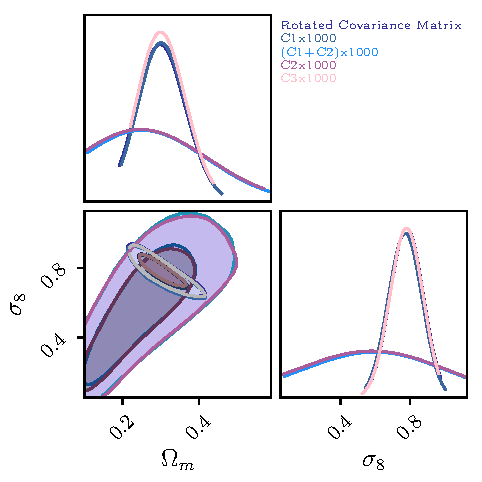
\includegraphics[width=0.9\columnwidth]{Multiply_error.pdf}
%		\caption{The upper right and lower left plots display the correlation matrix for BJ and CL respectively, while the lower right is the difference between the two. \label{fig:tolerance1000}}
%	\end{figure}
	
	
	
	%		In this section, we will introduce the methodology of tolerance testing on the covariance matrices in the new basis. We will show that after the basis transformation, we need to compare tremendously less elements from two covariance matrices.
	
	%	Generally speaking, the parameter constraints will get wider when part of the covariance matrix gets larger, because this means that the data is worse measured. In the normal basis, each data points varies with the parameter set, so the change of each element in the covariance matrix will affect the constraints. However, since we have found a basis where some of the data points change with parameter set while others do not, the elements that matters to the cosmological constraints will also shrink. To be specific, the C1 and C2 blocks in Figure~\rf{illu-trans} are the only parts that impact the parameter constraints. 
	
	%	In order to illustrate this statement, we will first perform a sanity check. We will make each of the blocks in the covariance matrices a large number and run a chain with that covariance. We run 3 tests by making
	%	1) C3,  
	%	2) C2, 
	%	3) C1 and C2,
	%	100 times of itself/themselves. In principle, we should see that the constraints for test 1 will not change but will get wider for test 2 and will totally blow up for test 3.
	
	%	Furthermore, we want to know how minor uncertainty on the informative elements of the covariance matrix will affect the cosmological constraints.
	
	% ----------------------------------------------------------------------
	% ----------------------------------------------------------------------
	
	
	% This work used some telescope which is operated/funded by some agency or consortium or foundation ...
	
	% We acknowledge the use of An-External-Tool-like-NED-or-ADS.
	
	%{\it Facilities:} \facility{LSST}
	
	% Include both collaboration papers and external citations:
	\bibliography{main}
	
\end{document}


% ======================================================================
